%% LaTeX source of the thesis.
%% Use command 'xelatex --shell-escape thesis.tex' TWICE to compile it into a PDF.

%%%%%%%%%%%%%%%%%%%%%%%%%%%%%%%%%%%%%%%%%%%%%%%%%%%%%%%%%%%%%%%%%%%%%%%%%%%%%%%%
% document preamble %%%%%%%%%%%%%%%%%%%%%%%%%%%%%%%%%%%%%%%%%%%%%%%%%%%%%%%%%%%%
%%%%%%%%%%%%%%%%%%%%%%%%%%%%%%%%%%%%%%%%%%%%%%%%%%%%%%%%%%%%%%%%%%%%%%%%%%%%%%%%
\documentclass[12pt, oneside, a4paper]{book}

\usepackage[UTF8]{ctex}			% for high level Chinese environment
\usepackage{caption}
\usepackage{enumerate}			% for customized list numbering
\usepackage{hyperref}			% for bookmarks and hyperlinks
\usepackage{amsmath}			% for mathematical features
\usepackage{amssymb}			% for mathematical symbols
\usepackage{amsthm}			% for theorems
\usepackage[chapter]{algorithm}		% for floated algorithm environment
\usepackage{algorithm}
\usepackage{algorithmic}
\usepackage{algorithmicx}		% for enhanced algorithm features
\usepackage{algpseudocode}		% for pseudo code algorithms
\usepackage{svg}			% for svg images
\usepackage{listings}			% for source code listing
\usepackage{color}			% for customized colors
% \usepackage{showframe}			% for showing page frames
\usepackage[BITstyle]{bitbook}		% for BIT-style thesis

% hyperref options
\hypersetup{
	% hide links
	hidelinks,
	% number bookmarks
	bookmarksnumbered = true,
	% fit width
	pdfstartview = {FitH},
	% PDF title
	pdftitle = {Zhuojia Shen's Undergraduate Thesis},
	% PDF subject
	pdfsubject = {Research in Embedding of Hypercubes into Circles},
	% PDF author
	pdfauthor = {Zhuojia Shen},
	% PDF keywords 
	pdfkeywords = {Hypercube; Circular embedding; Wirelength problem; Distributed computing}
}

% theorems
\newtheorem{theorem}{定理}[chapter]
\newtheorem{lemma}{引理}[chapter]

% algorithm settings
\floatname{algorithm}{算法}
\renewcommand{\algorithmicrequire}{\textbf{输入:}}
\renewcommand{\algorithmicensure}{\textbf{输出:}}

% svg options
\setsvg{
	svgpath = {./images/},		% svg directory
	inkscape = {inkscape -z -D}	% Inkscape command
}

% listings settings
\definecolor{commentgreen}{rgb}{0, 0.6, 0}
\definecolor{stringbrown}{rgb}{0.75, 0.5, 0}
\lstset{
	basicstyle = \ttfamily\footnotesize,
	tabsize = 2,
	showstringspaces = false,
	% highlight styles
	commentstyle = \color{commentgreen},
	keywordstyle = \color{blue},
	stringstyle = \color{stringbrown}
}

% BIT-style
\pagestyle{thesisbit}
\tocdepth{3}

% ctex settings
% \ctexset{
% 	chapter = {
% 		number = \arabic{chapter},
% 		format = \bfseries\songti\zihao{3}
% 	},
% 	section = {
% 		% number = \arabic{chapter},
% 		format = \bfseries\songti\zihao{4}
% 	},
% 	subsection = {
% 		format = \bfseries\songti\zihao{-4}
% 	}
% }


% list of files to include
\includeonly{
	abstract,
	chapter-1,
	chapter-2,
	chapter-3,
	chapter-4,
	chapter-5,
	chapter-6,
	acknowledgements,
	bibliography,
	appendices
}

%%%%%%%%%%%%%%%%%%%%%%%%%%%%%%%%%%%%%%%%%%%%%%%%%%%%%%%%%%%%%%%%%%%%%%%%%%%%%%%%
% document body %%%%%%%%%%%%%%%%%%%%%%%%%%%%%%%%%%%%%%%%%%%%%%%%%%%%%%%%%%%%%%%%
%%%%%%%%%%%%%%%%%%%%%%%%%%%%%%%%%%%%%%%%%%%%%%%%%%%%%%%%%%%%%%%%%%%%%%%%%%%%%%%%
\begin{document}

\zihao{-4}\ziju{0.1}
\baselineskip 22pt

%% LaTeX source of Abstract of the thesis.
%% NEVER compile this file. Complie 'thesis.tex' instead.

\chapter*{摘要}
\label{Abstract CN}
时序数据是按时间索引的一系列数据,例如汽车引擎中各类传感器采集到的数据,其中包括油量,速度,喷油量等。这类时序数据通常维数较高,体量较大。高体量意味着海量的时序数据将对存储系统造成很大的压力,而高维度意味着我们必须采用特殊的压缩算法来解决多维度的数据压缩难题并保证可靠的效率。因此本论文先通过特定的数据压缩算法实现多维度数据压缩,并将压缩后的数据进行持久化,同时为了方便直观的提取时序数据压缩过后包含的关键信息,我们使用蜡烛图来进行时序数据的可视化。
\hfill\break

\textbf{关键词:} 时序数据;数据压缩;持久化;可视化;蜡烛图

\chapter*{Abstract}
\label{Abstract EN}

Time-series data is a collection of data indexed by time sequence.Various types of data such as a car engine sensor to include oil, speed, fuel injection quantity and the like. Such time-series data is usually higher dimension, a larger volume. High volume means massive time-series data storage system will cause great pressure, and high-dimensional means that we must use special compression algorithms to solve multi-dimensional data compression problems and ensure reliable efficiency. Therefore, this paper first compressed data through a specific algorithm to achieve multi-dimensional data compression, data and compressed for persistence, in order to facilitate intuitive view of the time-series data compression result we use candles to visualize.
\hfill\break

\textbf{Keywords:} Time-series Data; Data Compression;Persistence;Visualization;Candlestick Charts

\tableofcontents
%% LaTeX source of Chapter 1 of the thesis.
%% NEVER compile this file. Complie 'thesis.tex' instead.

\chapter{引言}
\label{Chapter 1}

时序数据是按时间节点进行记录的数据集合,与非时序数据相比,它的顺序性要求更高,数据的应用范围更广。时序数据产生于生活中的各个方面,例如气
象观测中的大气数据、汽车发动机的各项传感器数据。这类数据不仅维度很高,同时产生的数据体量也非常大。目前随着时序数据规模的增大,不加处理的
原始数据已经对关系数据库特别是对一些移动平台和其它嵌入式设备造成了很大的存储压力。由于时序数据在一定时间内的重复率比较高,例如汽车的速度
在某段时间内都保持在一定速度,油料温度也都稳定在一定范围内,特别是对于发动机磨粒浓度这类数据很有可能长时间都稳定在某固定值,此类数据导致
了存储空间的严重浪费。高维时序数据是时序数据在空间上的扩展,相比于一维数据,多维时序数据复杂度更高,数据要求的存储空间更大。

理想的数据压缩效果是实现最小的存储成本,提高数据的传输效率。随着云计算和物联网的不断发展,数据的压缩存储技术成为海量数据研究的重要内容,根据
数据压缩后是否能完全还原为原始数据我们将数据压缩分为有损压缩和无损压缩,无损压缩的期望压缩比通常在1/2到1/5,相对于无损压缩,有损压缩
通常只要求压缩后的数据不影响特定范围内的正常使用,有损压缩广泛运用于视频和音频的压缩。

单维时序数据已经存在很多的成熟的压缩算法,例如SDT算法。相比于单维时序数据多维时序数据的压缩更为复杂,但是生活中需要对高维时序数据进行压
缩的场合却是很多,目前存在一些针对于时序数据的压缩算法,例如旋转门,稳态阈值,线性外插值等压缩算法,但是大多属于一维数据的有损压缩算法,
不能直接运用于多维时序数据的数据压缩,而且这些压缩算法的复杂度过高,海量的数据更是需要庞大的计算资源,而且这些压缩数据压缩后不能直接存储于关系数据库,这很大程度的影响了这些数据对于业务的使用。因此本论文设计了一种针对于高维时序数据的压缩方法,并提供了一种附加的持久化方式。

对于压缩处理过后的时序数据如何快速的从中找到自己需要的信息这是一个比较通用的业务场景,数据可视化的目的就是将这些晦涩难懂的数据在与用户的交互中展示出来。可视化的图表,更易于我们观察,对于发现数据的特征和深入的理解数据隐含的行为有更大的帮助,数据可视化不同于将所有的数据通过图标直接显示,数据体量超大的时序数据,直接用可视化系统观测不仅对可视化系统造成了巨大的压力,更重要的是这通常会直接导致高价值的数据被淹没。

根据现有的绝大部分业务场景,一般的持久化都是采用的基于关系操作的关系数据库,例如PC端常用的MySQL,移动端广泛运用的SQLite,当然也不排除一些特殊的业务场景使用了类似于MongoDB的非关系数据库。在本论文中我们给出了一种基于蜡烛图的的海量时序数据的可视化方法,具体的可视化我们使用开源的图形化报表库,在可视化的过程中我们先对时序数据进行高效的线性压缩,生成特定的区间,对于每个区间的统计数据,我们采用折线图和蜡烛图进行可视化。这种方法不仅能够对原始数据进行大范围的压缩,还能在压缩的基础之上通过用户的需求分层显示压缩后的效果

本论文依次介绍了相关的应用历史背景,算法实现,程序的相关实现等其它步骤,并在最后给出了一些针对于特定场合的压缩选项和优化。








%% LaTeX source of Chapter 2 of the thesis.
%% NEVER compile this file. Complie 'thesis.tex' instead.

\chapter{预备知识}
\label{Chapter 2}

\section{数据压缩简介}
\label{Section 2.1}


数据压缩的一般前提是不损失有用信息,理想的效果是达到最小的存储空间,同时提高传输和存储的效率。我们通过一定的算法重新组织数据,从而来减少
数据的冗余。数据压缩可分成两种类型,一种叫做无损压缩,另一种叫做有损压缩。无损压缩通常能保证在压缩数据后我们可以通过目标数据进行重构,
重构出的数据能和原始数据保持一致。常见的无损压缩包括磁盘文件的压缩,无损压缩的效果一般能把普通文件的数据压缩到原来的1/2到1/5.常用的
无损压缩算法包括霍夫曼算法,LZW(Lenpel-Ziv\&Welch)压缩算法。有损压缩是指在压缩后我们可以通过目标数据重构出原始数据的主要轮廓而这些
数据不会影响到我们对他们的使用。


\section{数据压缩的理论极限}
\label{Section 2.2}

了解了2.1中数据压缩的概念和相关分类,我们给出数据压缩的理论极限,值得一提的是对于时序数据的数据点压缩也存在压缩极限当数据压缩到一定程度之后,再提高压缩比例,带来的结果就是数据的永久性损害。

假设在均匀分布的情况下,我们采集到的某一维数据的取样值在存储文件中出现的概率是p,那么在这个取样值最多可能出现1/p种情况。因此我们需要log$_{2}$(1/p)
个存储单位表示该采样数据。我们把这个结论可以推广到一般情况。假设我们采样的某一维时序数据由n个采样值组成,每个部分的内容在存储文件中的出现概率分别为
p1、p2、...pn。那么,替代符号占据的存储单位最少为下面这个表达式:
\begin{equation}
$log_{2}(1/p1) + log_{2}(1/p2) + ... + log_{2}(1/pn)= \sum_{1}^{n}log_{2}(1/pn)$
\end{equation}
考虑单个采样值,它对应的存储单位为:
\begin{equation}
∑ log_{2}(1/pn) / n= log_{2}(1/p1)/n + log_{2}(1/p2)/n + ... + log_{2}(1/pn)/n
\end{equation}


\section{蜡烛图}
\label{Section 2.3}
蜡烛图(candlestick charts)也叫K线图,蜡烛图来源于对统计数据的分析,例如股价,其中包含股价的开盘价,收盘价,最高价和最低价。

K线图的状态可以分为翻转形态,整理形态等。K线图由于其细致明确的表达效果,引入到了股市和期货市场,K线图由统计区间的开始值,最大值,最小值,结束值组
成,假设给定一个统计区间,当我们确定区间的开始值和结束值时,我们把这两者中间的部分用对应的实体矩形画出,当开始值小于结束值时,我们用红色标注,此时K线被称为阳线,当开始值大于结束值时我们用黑色标注,此时对应的K线我们称之为阴线。

K线图绘制的技术指标和K线图的分析对于我们从中寻找有用的数据有很大的帮助。它可以作为我们从时序数据中寻找奇点数据最有力的工具,根据经典的K线图或者图上的某一指标分析和得出的结论不一定完全正确,但是结合我们时序数据压缩过后的数据查询,就能准确而快速的寻找到问题所在。

\textbf{注意:}时序数据绘制过程中的技术指标是对应于某一段时间内的统计分析数据,并不是和原始数据完全一样。因此这些数据的最终效果可能会受到人为因素
的控制,例如我们设置的压缩比过大,那么此时的绘图界面可能和原始数据相差较大。此时我们应该结合主要因素来判断图形是否能表达原始数据的真实趋势,以及我
们是否需要调整原始数据的压缩比和其它参数,以达到理想的效果。

\section{JavaScript\&Echarts}
\label{section 2.4}
JavaScript是一种直译式脚本语言,是一种动态类型、弱类型、基于原型的语言,内置支持类型。它的解释器被称为JavaScript引擎,为浏览器的一部分,广泛用于客户端的脚本语言,最早是在HTML(标准通用标记语言下的一个应用)网页上使用,用来给HTML网页增加动态功能。

HTML5的设计目的是为了在移动设备上支持多媒体。新的语法特征被引进以支持这一点,如video、audio和canvas标记。HTML5还引进了新的功能,可以真正改变用
户与文档的交互方式,包括:\newline
\begin{itemize}
 \setlength{\itemsep}{1pt}
 \setlength{\parskip}{0pt}
 \setlength{\parsep}{0pt}
 \item 新的解析规则增强了灵活性
 \item 淘汰过时的或冗余的属性
 \item 一个HTML5文档到另一个文档间的拖放功能
 \item 多用途互联网邮件扩展(MIME)和协议处理程序注册
 \item 在SQL数据库中存储数据的通用标准(Web SQL) 
\end{itemize}

JavaScript\&CSS\&HTML.是前端开发的必备工具,JavaScript作为事件处理和交互的核心起到了重要的作用,在HTML5中新增了canvas元素,这为我们绘制高质
量的蜡烛图提供了一个非常不错的选择,结合使用百度提供的echarts图形化报表组件,能够快速高质量的帮助我们完成工作。当然作为绘图工具。你依然可以选择其
它的工具,例如基于Java Swing的UI组件库,也可以选择基于Matlab的绘图套件,不过这些工具不一定适合在工程下的业务环境。



\section{JAVA\&设计模式}
\label{Section 2.5}

高维时序数据压缩的研究成果适用于工程中的很多场景,而Java语言也是现阶段业务场合中使用最为频繁的编程语言,论文的设定环境为基于Java 
EE虚拟机的嵌入式平台,因此需要了解Java EE相关的一些基础知识。


JDBC是Java 语言中与数据库交互最为流行的方式,绝大部分数据库都有特定的JAR包来实现这些接口。而现在最流行的持久化框架包括Hibernate,Ibatis都是基
于JDBC完成的,学会使用JDBC是完成该论文的重点。

设计模式(Design Pattern)是一套反复被使用,多数人知晓,经过分类与编目的代码设计经验的总结,使用设计模式的目的是使代码的可用度达到最大化,同时使用良好的设计模式对于代码的维
护也有很重要的作用,在本论文中需要了解的设计模式包括线程安全的单例模式,工厂模式,原型模式,和装饰者模式以及访问者模式。









%% LaTeX source of Chapter 3 of the thesis.
%% NEVER compile this file. Complie 'thesis.tex' instead.

\chapter{历史研究}
\label{Chapter 3}

\section{边等周问题}
\label{Section 3.1}

在图论中,大量的问题都可以被转化为边等周问题并得到解决,包括一些图嵌入问题。
在 L. H. Harper 的著作 \cite{Harper.1964,Harper.2004} 中,
他通过一系列的转化,利用边等周问题证明了从超立方体到链嵌入的线长问题。

下面我们给出边等周问题的定义,
再简要概述如何利用其解决从超立方体到链嵌入的线长问题,
并给出 $Q_d$ 上的边等周问题证明过程的改进。
注意这种转化方式为我们提供了一种重要的问题解决思路。

\subsection{定义}
\label{Subsection 3.1.1}

对于任意的图 $G$ 和 $S \subseteq V_G$,令
\begin{equation*}
\Theta(S) = \{e \in E_G \colon \partial_G(e) = \{v, w\}, v \in S, w \notin S\}
\end{equation*}
并称之为 $S$ 的\emph{边界}(Edge-boundary)。
那么对于一个给定的图 $G$ 和自然数 $k$,
\emph{边等周问题}(Edge-Isoperimetric Problem, EIP)
是对于所有的 $S \subseteq V_G$ 并且 $|S| = k$,寻找
\begin{equation*}
\min_{|S| = k} |\Theta(S)|
\end{equation*}
和能达到该最小值的子集 $S$。

为了便于下文叙述,我们在这里定义一个与 EIP 类似的问题,
并给出其在 $Q_d$ 下与 EIP 的关系。

对于任意的图 $G$ 和 $S \subseteq V_G$,令
\begin{equation*}
E(S) = \{e \in E_G \colon \partial_G(e) = \{v, w\}, v \in S, w \in S\}
\end{equation*}
并称之为 $S$ 的\emph{导出边集}(Induced Edges)。
对于一个给定的图 $G$ 和自然数 $k$,
\emph{导出边问题}(Induced Edge Problem)
是对于所有的 $S \subseteq V_G$ 并且 $|S| = k$,寻找
\begin{equation*}
\max_{|S| = k} |E(S)|
\end{equation*}
和能达到该最大值的子集 $S$。

\begin{lemma}
\label{Lemma 3.1}
如果图 $G = (V_G, E_G, \partial_G)$ 是一个 $\delta$ 度正则图,
那么对于 $\forall S \subseteq V_G$,都有
\begin{equation*}
|\Theta(S)| + 2 |E(S)| = \delta |S|
\end{equation*}
\end{lemma}

\begin{proof}[证明]
$\delta |S|$ 表示 $S$ 对应的边数,然而出现在 $E(S)$ 中的边被计算了两次。
\end{proof}

根据引理 \ref{Lemma 3.1},我们可以知道 $Q_d$ 上的导出边问题与 EIP 等价,
因为对于 $\forall S \subseteq V$ 和 $\forall k$,
$\min_{|S| = k} |\Theta(S)| = k d − 2 \max_{|S| = k} |E(S)|$。

\subsection{线长问题到 EIP}
\label{Subsection 3.1.2}

回想一下,
对于给定的编号方式 $\eta \colon V_{Q_d} \rightarrow V_{P_n}$,
在 $\eta$ 下从 $Q_d$ 到 $P_n$ 的线长 $wl(Q_d, P_n, \eta)$ 为
\begin{equation*}
wl(Q_d, P_n, \eta) = \sum_{\substack{
	e \in E \\
	\partial(e) = {v, w}
}} d_{P_n}(\eta(v), \eta(w)) = \sum_{\substack{
	e \in E \\
	\partial(e) = {v, w}
}} |\eta(v) - \eta(w)|
\end{equation*}
而从 $Q_d$ 到 $P_n$ 的线长问题则是寻找
\begin{equation*}
wl(Q_d, P_n) = \min_\eta wl(Q_d, P_n, \eta)
\end{equation*}

为了将从 $Q_d$ 到 $P_n$ 的线长问题转化为 $Q_d$ 上的 EIP,首先我们令
\begin{equation*}
S_k(\eta) = \eta^{-1}(\{0, 1, \dots, k - 1\}) = \{v \in V \colon \eta(v) \le k\}
\end{equation*}
即编号方式 $\eta$ 下的前 $k$ 个顶点的集合。
接下来,我们令
\begin{equation*}
\chi(e, k) = \begin{cases}
	1 & \text{如果}\ \partial(e) = \{v, w\}, \eta(v) \le k < \eta(w) \\
	0 & \text{其他情况}
\end{cases}
\end{equation*}
那么我们就有
\begin{align*}
wl(Q_d, P_n, \eta) & = \sum_{\substack{
			       e \in E \\
			       \partial(e) = \{v, w\}
		       }} |\eta(v) - \eta(w)|
		     = \sum_{e \in E} \sum_{k = 0}^n \chi(e, k) \\
		   & = \sum_{k = 0}^n \sum_{e \in E} \chi(e, k)
		     = \sum_{k = 0}^n |\Theta(S_k(\eta))|
\end{align*}
因此,
\begin{align*}
wl(Q_d, P_n) & = \min_{\eta} wl(Q_d, P_n, \eta) \\
	     & = \min_{\eta} \sum_{k = 0}^n |\Theta(S_k(\eta))| \\
	     & \ge \sum_{k = 0}^n \min_{\eta} |\Theta(S_k(\eta))|
	       = \sum_{k = 0}^n \min_{|S| = k} |\Theta(S)|
\end{align*}
根据该式,我们可以得到一个结论。

\begin{theorem}
\label{Theorem 3.1}
对于 $\forall \eta \colon V_{Q_d} \rightarrow V_{P_n}$,
如果它的所有初始段 $S_k(\eta)$($0 \le k \le n$)都是 EIP 的解,
那么它本身就是从 $Q_d$ 到 $P_n$ 的线长问题的一个解。
\end{theorem}

根据定理 \ref{Theorem 3.1},我们将问题转化为了 EIP。

\subsection{EIP 证明的改进}
\label{Subsection 3.1.3}

对于 $Q_d$ 上的 EIP,
L. H. Harper 在一篇论文 \cite{Harper.1964} 中提出了下面这个定理,
并给出了他的证明。

\begin{theorem}
\label{Theorem 3.2}
$S \subseteq V_{Q_d}$ 在基数为 $k$ 时有最大的 $|E(S)|$,当且仅当 $S$ 是立方集。
\end{theorem}

在定理 \ref{Theorem 3.2} 的证明过程中,
Harper 对 $d$ 进行数学归纳,并用到了下面这个性质:
如果 $2^{d - 1} \le k < 2^d$,那么
\begin{equation*}
E(k + 1) - E(k) = E(k - 2^{d - 1} + 1) - E(k - 2^{d - 1}) + 1
\end{equation*}
其中 $E(k)$ 表示一个 $k$-立方集 $S$ 的导出边数 $|E(S)|$,
因为 $|E(S)|$ 并非由 $d$ 决定,而仅仅由 $k = |S|$ 决定。

在这篇论文发表两年后,
A. J. Bernstein 发表了一篇后续论文 \cite{Bernstein.1967},
指出 Harper 忽视了一种情况。
他在这篇后续论文中提出了下面这个引理,用该引理修补了 Harper 的证明中的漏洞:

\begin{lemma}
\label{Lemma 3.2}
对于 $\forall d$ 和 $\forall k, t > 0$ 使得 $k + t < 2^d$,都有
\begin{equation*}
E(t) < E(k + t) − E(k) < E(2^d) − E(2^d − t)
\end{equation*}
\end{lemma}

在引理 \ref{Lemma 3.2} 的证明过程中,Bernstein 对 $d$ 进行数学归纳,
然后分别考虑了三种情况:
\begin{enumerate}[(1)]
	\item 当 $k \ge 2^{d − 1}$ 时,左右两边不等式成立;
	\item 当 $k + t \le 2^{d − 1}$ 时,左右两边不等式成立;
	\item 当 $k < 2^{d - 1} < k + t$ 时,左右两边不等式成立。
\end{enumerate}

然而我们发现第 3 种情况的证明依然存在纰漏:
Bernstein 并未考虑 $t \ge 2^{d − 1}$ 的情况,
即当 $k < 2^{d − 1} < k + t$ 时,
\begin{equation*}
E(2^{d − 1}) − E(k) > E(t) − E(t − (2^{d − 1} − k))
\end{equation*}
仅对 $t < 2^{d - 1}$ 成立。
下面我们给出经过补充的情况 3 的完整证明。

\begin{proof}[引理 \ref{Lemma 3.2} 情况 3 的完整证明]
当 $k < 2^{d − 1} < k + t$ 时,
\begin{enumerate}[(1)]
	\item 如果 $t \ge 2^{d - 1}$,那么对于左边的不等式,我们有
		\begin{align*}
		E(k + t) - E(k) & = \left[E(k + t) - E(2^{d - 1})\right] +
				    \left[E(2^{d - 1}) - E(k)\right] \\
				& = \left[E(k + t - 2^{d - 1}) + k + t - 2^{d - 1}\right] +
				    \left[E(2^{d - 1}) - E(k)\right] \\
				& = \left[E(k + t - 2^{d - 1}) - E(k)\right] +
				    E(2^{d - 1}) + k + t - 2^{d - 1} \\
				& > E(t - 2^{d - 1}) + E(2^{d - 1}) + t - 2^{d - 1} + k \\
				& = E(t) + k > E(t)
		\end{align*}
		对于右边的不等式,我们有
		\begin{align*}
		E(k + t) - E(k) & = \left[E(k + t) - E(2^{d - 1})\right] +
				    \left[E(2^{d - 1}) - E(k)\right] \\
				& = \left[E(k + t - 2^{d - 1}) + k + t - 2^{d - 1}\right] +
				    \left[E(2^{d - 1}) - E(k)\right] \\
				& = \left[E(k + t - 2^{d - 1}) - E(k)\right] +
				    E(2^{d - 1}) + k + t - 2^{d - 1} \\
				& < E(2^{d - 1}) - E(2^d - t) + E(2^{d - 1}) +
				    k + t - 2^{d - 1} \\
				& = 2 E(2^{d - 1}) + k + t - 2^{d - 1} - E(2^d - t) \\
				& < 2 E(2^{d - 1}) + 2^{d - 1} - E(2^d - t) \\
				& = E(2^d) - E(2^d - t)
		\end{align*}
	\item 相应地,如果 $t < 2^{d - 1}$,那么对于左边的不等式,我们有
		\begin{align*}
		E(k + t) − E(k) & = \left[E(k + t) − E(2^{d − 1})\right] +
				    \left[E(2^{d − 1}) - E(k)\right] \\
				& = \left[E(k + t - 2^{d - 1}) + k + t - 2^{d - 1}\right] +
				    \left[E(2^{d - 1}) - E(k)\right] \\
				& > E(k + t - 2^{d - 1}) +
				    \left[E(t) − E(t − (2^{d − 1} − k))\right] \\
				& = E(t)
		\end{align*}
		对于右边的不等式,我们有
		\begin{align*}
		E(k + t) - E(k) & = \left[E(k + t) - E(2^{d - 1})\right] +
				    \left[E(2^{d - 1}) - E(k)\right] \\
				& = \left[E(k + t - 2^{d - 1}) + k + t - 2^{d - 1}\right] +
				    \left[E(2^{d - 1}) - E(k)\right] \\
				& = \left[E(k + t - 2^{d - 1}) - E(k)\right] +
				    E(2^{d - 1}) + k + t - 2^{d - 1} \\
				& < E(2^{d - 1}) - E(2^{d - 1} - t) + t + k - 2^{d - 1} \\
				& = E(2^d) - E(2^d - t) + k - 2^{d - 1} \\
				& < E(2^d) - E(2^d - t)
		\end{align*}
\end{proof}

\section{Guu 的研究与缺陷}
\label{Section 3.2}

待撰写。

\section{边拥塞与分区引理}
\label{Section 3.3}

待撰写。

%% LaTeX source of Chapter 5 of the thesis.
%% NEVER compile this file. Complie 'thesis.tex' instead.

\chapter{程序设计与实现}
\label{Chapter 4}

\section{开发环境介绍}
\label{4.1}
\begin{enumerate}[(1)]
	\item 开发环境:eclipse
	\item 持久化:SQLite
	\item 项目构建工具:Maven
	\item 语言:Java\&JavaScript
\end{enumerate}

\section{需求分析}
\label{4.2}
\begin{enumerate}[(1)]
	\item 基于B/S 完成整个项目。
	\item 实现数据压缩算法,并绘制相应的可视化界面。
	\item 实现压缩选项参数的可定制化。
	\item 实现灵活可扩展的接口设计,能实现持久化平台和可视化工具的自由切换。
	\item 保证代码的可维护性,尽可能多的合理准确的增加对相应设计模式的使用。
	\item 通过代码实现,验证算法的可行性,并对算法给出改进。
\end{enumerate}

\section{时序数据模拟设计}
\label{4.3}
\subsection{时序数据模拟器接口}
业务场景中时序数据来自于物理数据,这些数据具有真实的物理特性,在压缩过程中更能体现出压缩算法的效果。在本论文的实现过程中我们采用了相关的模拟时序
算法来生成一些时序数据,这些数据能较好的达到压缩的基本需求。对于一个时序数据模拟器接口,设计时最需要考虑的就是时序数据的接口的合理性,好的时序数据接口能以很少的更改,直接切换到真实的时序数据来源,同时还要降低对我们代码的侵入性,因此一个时序数据接口仅仅包含产生时序数据,时序数
据开始和停止三个方法,任何时序数据接口的实现都必须完全实现这三个方法。我们设计的接口显示如下:
\begin{lstlisting}
public interface DataGen{
	public ArrayList<?> getGenData();
	public void run();
	public void stop();
}
\end{lstlisting}
注:DataGen接口含有一个模拟器的所有方法,一个模拟器的实现必须至少含有这些方法。



\subsection{时序数据模拟器工厂}
用户在时序数据压缩的过程中,首先会运行时序数据模拟器,但是用户完全不用知道时序数据模拟器是如何产生的,此时我们引入了时序数据模拟器的抽象工厂,该工
厂最大限度的隐藏了时序数据模拟器。并实现了更高程度的代码分离。
\begin{lstlisting}
public class DataGenFactory{
	public DataGen createDataGen();
}
\end{lstlisting}
注:DataGenFactory工厂提供出一个时序数据模拟器实例,调用者只需要查看DataGen的接口代码即可,不用关心DataGen的具体实现。


\subsection{持久化JDBC链接}
\begin{lstlisting}
public abstract class Instance{
	public void connection();
	public void startTransaction();
	public void insert();
	public void delete();
}
\end{lstlisting}
注:时序数据持久化类为抽象类,必须提供事务操作。



\subsection{时序数据模拟实现}
\begin{lstlisting}
public class SeriesDataGen implements DataGen{
	@override
	public ArrayList<?> getGenData();
	@override
	public void run();
	@override
	public void stop();

	private ArrayList arrayList;

	pivate createdate();//该方法产生对应的数据

	public static getDataGen(){//此处使用了一个单例模式
		if(dataGen==null)
			dataGen=new DataGen()
		
		return dataGen;
	}

	private static DataGen dataGen;
}
\end{lstlisting}
注:由于篇幅限制,我们给出了时序数据的产生接口设计,同时我们在上述过程中使用了工厂和单例的设计模式。




\section{数据压缩处理}
\label{4.4}
\subsection{时序数据压缩接口}
时序数据压缩的整个过程,可以分为三个阶段,其中包括时序数据的区间产生,时序数据的区间合并,还有时序数据的最终生成这三个过程,由于这三个过程紧密结合,具有较高程度的耦合性,没有其它的需求需要单独调用这三个方法,因此我们通过一个process来完成这所有的操作,并且我们将这三个处理类设计为受保护类型,因此他们的可见性,都停留在自己的包命名空间之内。
\begin{lstlisting}
public class DataCompress{
	private process(ArrayList<?> dataarray){

	}
	public void CompressInterval();//此方法为直接调用方法

	private void IntervalMerage();//区间合并算法

	private void getGenData();//数据生成算法

	public void react();//此方法为注册方法

}
\end{lstlisting}
注:此类包含了一个数据处理的单个过程。


\subsection{时序数据处理中心}
\begin{lstlisting}
public class processcore{
	private List<DataCompress> list;

	public void register(DataCompress unit);

	private listIterator;
}
\end{lstlisting}

注:此类包含了各个处理类的注册中心,当processCore接受到特定消息,包括stop,suspend等
消息,就可以调用相应的react方法。这用到了迭代器和监听器模式。

\subsection{可视化的绘图}

盒图是在1977年由美国的统计学家约翰·图基(John Tukey)发明的。它由五个数值点组成:最小值(min),下四分位数(Q1),中位数(median),上四分位数(Q3)
,最大值,结合K线图。我们实现了这两者特点的结合,改进后的K线图显示如下。\ref{Figure 4-1-1}:

\begin{figure}[h!]
	\centering
	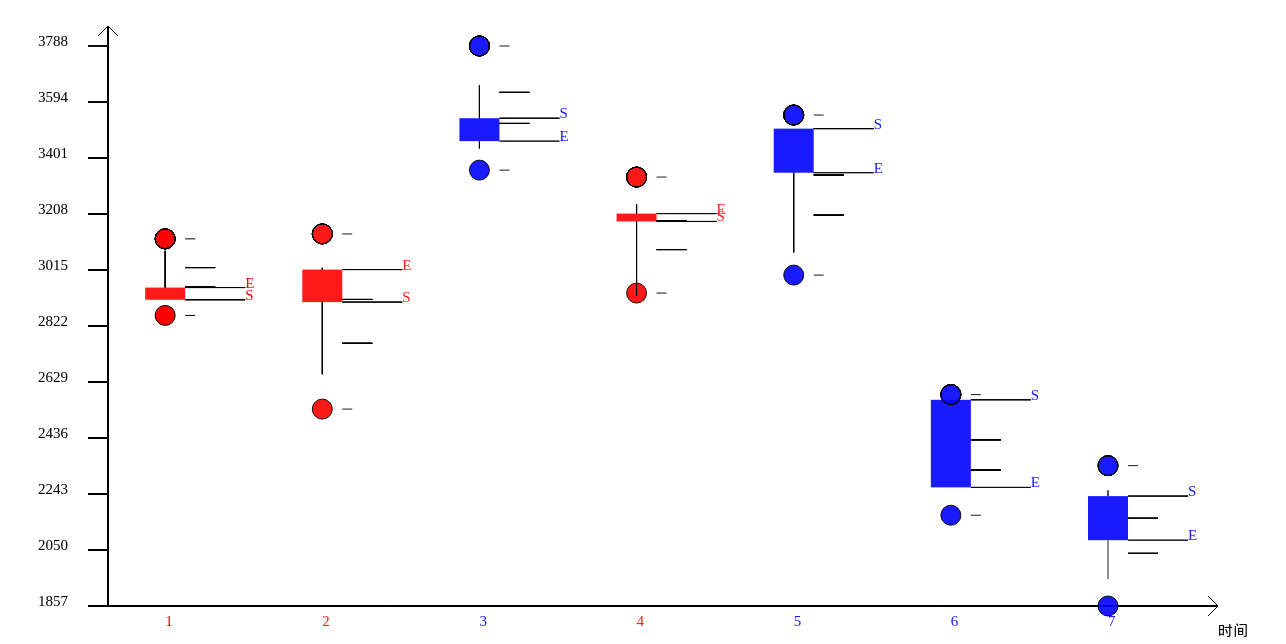
\includegraphics[scale=0.25]{./images/figure-4-1}
	\caption{时序输入数据}
	\label{Figure 4-1-1}
\end{figure}

























%% LaTeX source of Chapter 5 of the thesis.
%% NEVER compile this file. Complie 'thesis.tex' instead.

\chapter{结果分析}
\label{Chapter 5}

我们通过第三章给出的核心算法,以及第四章的需求和设计,来对时序数据压缩的情况进行模拟与分析。

\section{示例说明}
\label{5.1}
通过第四章的描述我们知道,压缩模拟的过程中,我们先通过模拟时序数据发生器,来生成时序数据,原始数据的产生时间间隔为10ms,当原始数据生成以后我们对每一个区间按照区间分隔算法来进行数据区间的分割,当区间分割完毕之后,我们通过数据区间的合并算法对那些数据点过密也就是区间内的数据点数超过限制的区间进行合并,然后我们通过数据生成算法来生成压缩后的数据。最后我们可以通过基于浏览器来显示我们的可视化数据。

\section{模拟过程}
\label{5.2}

\subsection{时序数据模拟产生}
\label{5.21}
在程序的实际实现过程中,数据的维数接近100,此处由于篇幅限制,我们将维数降低以使结果更加明显,程序运行的过程如图所示,\ref{Figure 5-1-1}此处我们将输出数据重定向到了活动窗口。

\begin{figure}[h!]
	\centering
	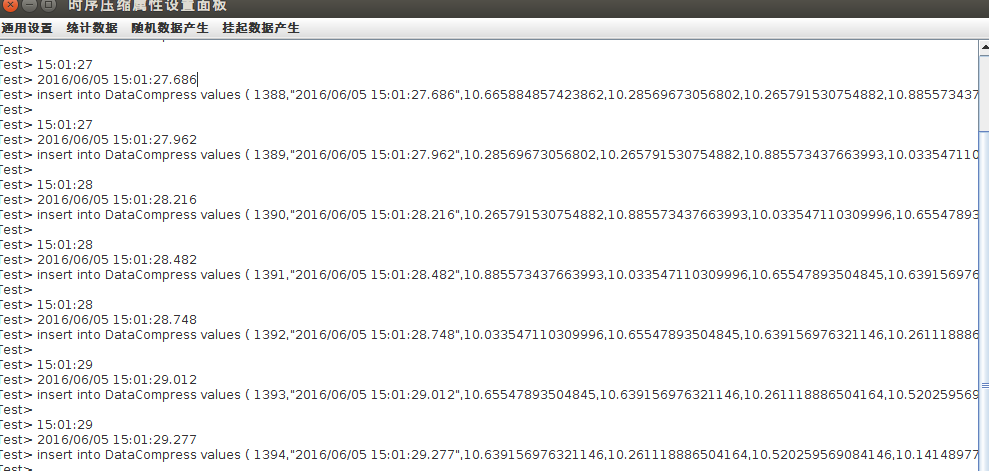
\includegraphics[scale=0.35]{./images/figure-5-1}
	\caption{模拟时序数据发生器}
	\label{Figure 5-1-1}
\end{figure}



如图对应的原始表如下:

\begin{center}
  \begin{tabular}{ | p{1.5cm} | p{1.5cm} | p{1.5cm} | p{1.5cm} | p{1.5cm} | p{1.5cm}|p{1.5cm}}
    \hline
    T  & D$_{1}$ & D$_{2}$ & D$_{3}$ & D$_{4}$  & D$_{5}$ &  D$_{6}$  \\ \hline
    1  & 10.6     & 10.2     & 10.2     & 10.8  &10.8     &   10.8     \\ \hline
    2  &10.2      &10.2      &10.8      &10.0   &10.0     &   10.0     \\  \hline
    3  &10.2      &10.2      &10.8      &10.0   &10.0     &   10.0      \\ \hline
    4 &10.8      &10.0      &10.0      &10.1    &10.0     &   10.0   \\ \hline
    5 &10.8      &10.0      &10.0      &10.1    &10.1     &   10.2    \\ \hline
    6 &10.7      &10.2      &10.2      &10.2    &10.0     &   10.2    \\ \hline
    7 &10.9      &10.2      &10.3      &10.2    &10.3     &   11.0     \\ \hline
    \hline
  \end{tabular}
\end{center}


\subsection{时序数据区间分隔}
\label{5.22}
通过原始数据的每一列我们进行区间划分,划分的规则如下:

\begin{lstlisting}
D1  [1,1]  [2,3]  [4,7]
D2  [1,7]
D3  [1,1]  [2,3]  [4,7]
D4  [1,1]  [2,7]
D5  [1,1]  [2,7]  
D6  [1,1]  [2,7]
\end{lstlisting}


\subsection{区间合并与数据生成}
\label{5.23}
由时序数据区间分隔算法产生的区间点包括[1,1],[2,3],[4,7],由这些时间点的生成的区间如下表所示:

\begin{center}
  \begin{tabular}{ | p{1.5cm} | p{1.5cm} | p{1.5cm} | p{1.5cm} | p{1.5cm} | p{1.5cm}|p{1.5cm}}
    \hline
    T  & D$_{1}$ & D$_{2}$ & D$_{3}$ & D$_{4}$  & D$_{5}$ &  D$_{6}$  \\ \hline
    1  & 10.6     & 10.2     & 10.2     & 10.8  &10.8     &   10.8     \\ \hline
    2  &10.2      &10.2      &10.8      &10.0   &10.0     &   10.0     \\  \hline
    3  &10.8      &10.1      &10.8      &10.1   &10.1     &   10.1      \\ \hline
    \hline
  \end{tabular}
\end{center}

\newpage 

\subsection{可视化示例}
\label{5.24}
时序数据通过可视化后的显示如下\ref{Figure 5-1-2},从图中我们可以观察到统计数据的开始值,结束值,最大值,最小值,以及分布情况。

\begin{figure}[h!]
	\centering
	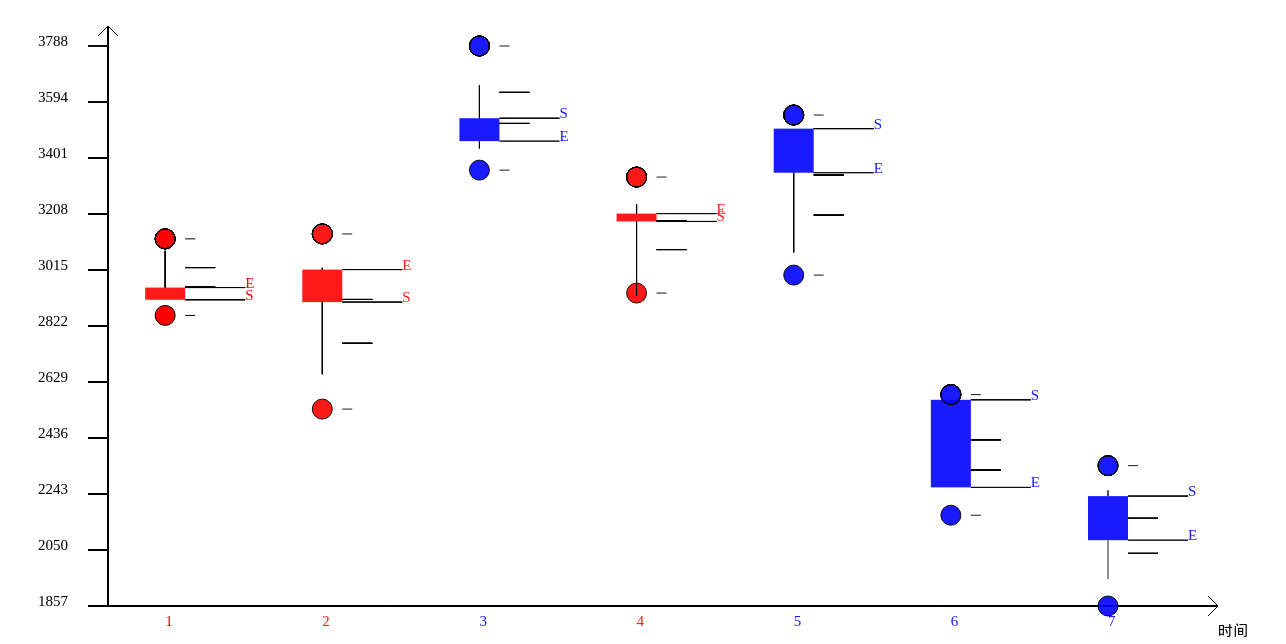
\includegraphics[scale=0.35]{./images/figure-5-2}
	\caption{模拟时序数据发生器}
	\label{Figure 5-1-2}
\end{figure}

图中包含以下有效信息:

\begin{enumerate}[(1)]
	\item 红颜色方块代表开始值大于结束值,蓝色方块为开始值小于结束值。
	\item 开始值和结束值被实体方块包围。
	\item 次短线代表3/4位数,和1/4位数。
	\item 最短线代表最大值和最小值。
\end{enumerate}





\subsection{压缩结果分析}
\label{5.25}
通过上述的过程我们可以看出,原始数据的时间点数为6,而压缩处理过后产生的时间点数为3,这在存储的过程
中减少了一半的存储量,这是在我们的波动误差约为0.5所得出的结论,如果我们的误差设置为1,那么压缩效果
可以达到1/6,由此可见,在条件允许的情况下,这能节省大量的存储空间。











%% LaTeX source of Chapter 6 of the thesis.
%% NEVER compile this file. Complie 'thesis.tex' instead.

\chapter{总结}
\label{Chapter 6}

从全文的整体结构来看,我们完成了高维时序数据压缩到可视化的一整套流程。首先我们介绍了时序数据的相关特征,时序数据压缩的相关历史研究,然后我们就时序
数据压缩所需要的工具与算法进行了介绍,在程序设计与实现部分我们给出了基于Java相关平台的设计与实现思路。在实验结果部分我们给出了压缩实例和压缩效果的
展示。

从压缩效果来看,本论文提供了一种切实可行的高维时序数据压缩的可选方案,从可视化的角度来看我们又提供了对于不同可视化工具的支持设计。我们的原则
是基于可扩展的接口设计,同时强调设计的可重复使用性。总体来说论文中的整体设计与实现是对高维时序数据与可视化的一次有益的探索。对于工程中的使用者来说我们的设计思路也有相当的参考价值。

\section{未来工作}
\label{Section 6.1}

针对高维时序数据压缩和可视化这一问题,以及我们的研究结果,
未来还有许多进一步的工作可以继续开展:
\begin{enumerate}[(1)]
	\item 在时序数据的压缩算法上我们应该还有很多需要改进的部分
	\item 时序数据压缩的计算量异常庞大,我们可以尝试基于分布式系统来提高我们的计算速度
	\item 如何构造一个更为准确的时序数据产生模型
	\item 对于压缩梯度的设置我们是否能够设计的更为准确
	\item 在程序设计部分离工程的标准还有一定的差距,我们应该以更为合理和优秀的设计为目标。
\end{enumerate}

%% LaTeX source of Acknowledgements of the thesis.
%% NEVER compile this file. Complie 'thesis.tex' instead.

\chapter*{致谢}

近半年的学习和科研工作不仅使我的知识结构和科研能力上了一个新台阶更重要的是各方面的素质得到了提高。而这一切都要归功于刘庆晖老师的深切教诲与热情鼓励
。值此论文顺利完成之际我首先要向我尊敬的导师刘庆晖老师表达深深的敬意和无以言表的感谢。同时感谢计卫星老师在我学习期间给予的帮助。感谢和我一起工作的
沈卓佳同学,张露露学姐。沈卓佳灵活考虑问题的方式严谨的解决问题的态度张露露学姐扎实的专业知识功底认真的科研态度都给我留下了深刻的印象。感谢和我同一实
验室的高志伟学长。没有他们无私的帮助我是无法完成论文工作的。感谢我的室友王天舒、沈卓佳、彭逸云和他们一起度过了这段美好时光是难以忘记的。 最后深深的
感谢呵护我成长的父母。每当我遇到困难的时候父母总是第一个给我鼓励的人。回顾20多年来走过的路每一个脚印都浸满着他们无私的关爱和谆谆教诲10年的在外求学
之路寄托着父母对我的殷切期望。他们在精神上和物质上的无私支持坚定了我追求人生理想的信念。父母的爱是天下最无私的最宽厚的爱。大恩无以言报惟有以永无止
境的奋斗期待将来辉煌的事业让父母为之骄傲。我亦相信自己能达到目标。












%% LaTeX source of Bibliography of the thesis.
%% NEVER compile this file. Complie 'thesis.tex' instead.

\begin{thebibliography}{99}

\bibitem{Rosen.2012}
	关云鹏,杨静.
	高维时序数据的相似搜索[J].贵州大学学报(自然科学版),2006/23(1):44-50.DOI:10.3959/j.jssn.1000-5269.2006.01.010

\bibitem{Harper.2004}
	王成山,王继东.
	基于能量阈值和自适应算术编码的数据压缩方法[J],电力系统自动化2004/28(24):56-60

\bibitem{Guu.1997}
	黄勇,吕涛.
	基于线性插值函数的遥测数据压缩[J],计算机工程与应用,2004,38(1640-42
\bibitem{Manuel.2009}
	段培勇,张枚,汤同奎等SDT算法及其在局域控制网络中压缩过程数据的应用[J],信息与控制,2002,31(2):132-135.DOI:10.3969/j.jssn.1002-
	0411.2002.02.008

\bibitem{Manuel.2011}
	刘玉葆,李启睿
	一种基于压缩策略的高维空间子空间skyline查询算法[J],计算机研究与发展,2013(s1):101-108

\bibitem{Opatrny.2000}
	游文杰,吉国力,袁明顺,高维少样本数据的特征压缩,计算机工程与应用,2006/17(1):49-50

\bibitem{Harper.1964}
	Mah R S H ,et al.Process trending with piecewise linear smoothing .Comput Chem Engng,1995,19(2):129-137

\bibitem{Erbele.2003}
	Gray R M Vector quantizatio .IEEE ASAP Magazine,Apr,1984,4-29
\bibitem{Bezrukov.2000}
	Macgregor JF.Statisti cal process control of multivariate process IFAC ADCHEM,Kyoto Japan 1994
\bibitem{Ji.2015}
	ABflag.j.Friegel.HP similary search ontime series based on threshold queries in: Proceedins of the 10thinternationl COnferece on Extending DatabaseTechnolog pp.276-294
\bibitem{Bernstein.1967}
	Abonyi clustering for fuzzing segmentation of multivariate time-series .Fuzzy sets and Systems Data Mining SSpecial lssue 149:39-56

\bibitem{Ahmad 5}
	Oliveira PCF Ahmd K 2004 summarization fo multiodal information in: Proceedings of the Fourth Internationa COnference on Language Resources and Evalutation vol 3.pp 1049-1052
\bibitem{zwir}
	ENrique EH 1999 Qualitative object description:inital reports of the exploration of the frontier. Proceedings of Joint EUROFUSE-SIC99 Interational Conferecne pp:489-490
\bibitem{Yin B K}
	Sidiropouls Johnson T.Jagadish H.V Faloutsos C Biliris A 2000 online data mining for co-evolving time sequeces in Proceedings of the 16th IEEE International Conference on Data Engineering pp:201-208
\bibitem{Yin}
	Yin Yang Q 2006 Intergratiing Hidden Markov Models and spectral analysis for sensory time series clustering in: Proceedings of the Fifth IEEE internationalConference on Data Mining pp:06-513
\bibitem{Yand}
	Yand.K.Yoon H.Shahabi C. 2005 Clever: a feature subset selection technique for multivariate time seies in procedings of the Ninth Pacific-Asia COnference on Knowledge Discovery and Data Mining pp:516-522
\bibitem{Yand}
	Yang K .Sha on the stationarity of multivariate time seies for correlation-based data analysis in proceedings of the fifth IEEE international conference on Data Mining pp:805-808
\end{thebibliography}













%% LaTeX source of Appendices of the thesis.
%% NEVER compile this file. Complie 'thesis.tex' instead.

\appendix{时序模拟和时序压缩}
\label{Appendix A}

\section{GenData.java}
\label{Section A.1}

\begin{lstlisting}[language = Java]
package cn.BITCS.DataBase;

import java.io.FileNotFoundException;
import java.sql.SQLException;
import java.util.ArrayList;
import java.util.Random;

public class DataGen
{
	private ArrayList<String> Array;
	
	public void Init()
	{
		int i=0;
		Array=new ArrayList<String> ();
		
		Array.add(0, "0");
		Array.add(1, "null");
		
		for(i=2;i<=5;i++)
		{
			Array.add(i, GenerateDouble().toString());
		}
		
		for(i=6;i<=7;i++)
		{
			Array.add(i, GenerateBoolean().toString());
		}
		
		Array.add(8, GenerateDouble().toString());
		
		for(i=9;i<=11;i++)
		{
			Array.add(i, GenerateBoolean().toString());
		}
		
		for(i=12;i<=51;i++)
		{
			Array.add(8, GenerateDouble().toString());
		}
		
		Array.add(52, GenerateInteger().toString());
		
		for(i=53;i<=57;i++)
		{
			Array.add(8, GenerateDouble().toString());
		}
		
		for(i=58;i<=63;i++)
		{
			Array.add(i, GenerateBoolean().toString());
		}
		
		for(i=64;i<=77;i++)
		{
			Array.add(i, GenerateDouble().toString());
		}
		
		Array.add(78, GenerateBoolean().toString());
		
		for(i=79;i<=87;i++)
		{
			Array.add(i, GenerateDouble().toString());
		}
		
	}
	
	private int i=0;
	
	public void Insert() throws SQLException, FileNotFoundException
	{
		InsertInto PreInsert=new InsertInto();
		PreInsert.insert(Array);
	}
	
	private Double GenerateDouble()
	{
		Random RandomNumber=new Random(1000);
		Double Number=RandomNumber.nextDouble()*1000;
		if(Number%1000>=970)
		{
			Number=Number%5+10.0;
		}
		else
		{
			Number=10.0+Number%1.0;
		}
		
		return Number;
		
	}
	
	private Integer GenerateBoolean()
	{
		Random RandomNumber=new Random();
		Integer Number=RandomNumber.nextInt();
		if(Number%1000>990)
			return 1;
		else return 0;
	}
	
	private Integer GenerateInteger()
	{
		Random RandomNumber=new Random();
		Integer Number=RandomNumber.nextInt();
		return Number%5;
		
	}
}
\end{lstlisting}

\clearpage

\clearpage
\section{Instance.java}
\label{Section A.2}

\begin{lstlisting}[language = Java]
package cn.BITCS.DataBase;
import java.sql.*;

public class Instance{
	public static void main(String[] args) {
			try {
				Class.forName("org.sqlite.JDBC");
				Connection conn =DriverManager.getConnection("jdbc:sqlite:info");
				Statement stat = conn.createStatement();
				stat.executeUpdate("drop table if exists people;");
				stat.executeUpdate("create table people (name, occupation);");
				PreparedStatement prep = conn.prepareStatement("insert into people values (?, ?);");

				prep.setString(1, "Gandhi");
				prep.setString(2, "politics");
				prep.addBatch();
				prep.setString(1, "Turing");
				prep.setString(2, "computers");
				prep.addBatch();
				prep.setString(1, "Wittgenstein");
				prep.setString(2, "smartypants");
				prep.addBatch();

				conn.setAutoCommit(false);
				prep.executeBatch();
				conn.setAutoCommit(true);

				ResultSet rs = stat.executeQuery("select * from people;");
				while (rs.next()) {
				  System.out.println("name = " + rs.getString("name"));
				  System.out.println("job = " + rs.getString("occupation"));
				}
				rs.close();
				conn.close();
			} catch (ClassNotFoundException e) {
				// TODO Auto-generated catch block
				e.printStackTrace();
			} catch (SQLException e) {
				// TODO Auto-generated catch block
				e.printStackTrace();
			}
		}
	}\end{lstlisting}

\section{Compress.java}
\label{Section A.3}

\begin{lstlisting}[language = Java]
package cn.BITCS.SeqDataPre;

import java.sql.Connection;
import java.sql.DriverManager;
import java.sql.ResultSet;
import java.sql.SQLException;
import java.sql.Statement;
import java.util.ArrayList;

public class Compress{
	
	public void VictorSet()
	{
		
	}
	
	public void Scanner(int i2) throws ClassNotFoundException, SQLException
	{
		Class.forName("org.sqlite.JDBC");
		Connection conn =DriverManager.getConnection("jdbc:sqlite:info");
		Statement stat = conn.createStatement();
		
	     ResultSet rs = stat.executeQuery("select count(*) from DataCompress" );
	     
	     

	     if (rs.next()) 
	       {
	            Count = rs.getInt(1); 
	       }
	     
	     String SqlStatement="select * from DataCpress";
	     
	     int i=0;
	     for(i=2;i<=88;i++)
	     {
	     
	     stat.executeUpdate(SqlStatement);
	     
	     rs=stat.executeQuery(SqlStatement);
	     
	     Area area=new Area();
	     
	     area.setStart(0);
	     
	     while(rs.next())
	     {
	    	 if(rs.getDouble(2)>11.0)
	    	 {
	    		 area.setOver(rs.getRow());
	    		 Array.add(area);
	    		 area=new Area();
	    	 }
	    	 
	    	 if(new Integer(area.getMax())<new Integer(rs.getString(i)))
	    	 {
	    		 area.setMax(rs.getString(i));
	    	 }
	    	 
	    	 if(new Integer(area.getMax())<new Integer(rs.getString(i)));
	    	 {
	    		 area.setMax(rs.getString(i));
	    	 }
	    	 
	    	 if(new Integer(area.getMin())>new Integer(rs.getString(i)))
	    	 {
	    		 area.setMin(rs.getString(i));
	    	 }
	     }
	    }
	     
	}
	
	public void insert() throws ClassNotFoundException, SQLException
	{
		Class.forName("org.sqlite.JDBC");
		Connection conn =DriverManager.getConnection("jdbc:sqlite:info");
		Statement stat = conn.createStatement();
		int i=0;
		
		
		
		while(Array.get(i) != null)
		{
			String Data=Array.get(i).getAverage();
			stat.executeQuery("insert into data"+Data);
		}
		
		
	}
	
	private ArrayList <Area> Array;
	
	private Integer Count;
	
}
\end{lstlisting}

\section{TextAreaOutputSteamTest.java}
\label{Section A.4}

\begin{lstlisting}[language=java]
package cn.BITCS.SeqDataPre;
import java.awt.BorderLayout;
import java.awt.event.ActionEvent;
import java.awt.event.ActionListener;
import java.io.PrintStream;
import javax.swing.*;

@SuppressWarnings("serial")
public class TextAreaOutputStreamTest extends JPanel {

   private JTextArea textArea = new JTextArea(15, 30);
   private TextAreaOutputStream taOutputStream = new TextAreaOutputStream(
         textArea, "Test");

   public TextAreaOutputStreamTest() {
      setLayout(new BorderLayout());
      add(new JScrollPane(textArea, JScrollPane.VERTICAL_SCROLLBAR_ALWAYS, 
            JScrollPane.HORIZONTAL_SCROLLBAR_NEVER));
      System.setOut(new PrintStream(taOutputStream));

      int timerDelay = 1000;
      new Timer(timerDelay , new ActionListener() {
         int count = 0;
         @Override
         public void actionPerformed(ActionEvent arg0) {

            // though this outputs via System.out.println, it actually displays
            // in the JTextArea:
            System.out.println("Count is now: " + count + " seconds");
            count++;
         }
      }).start();
   }

   private static void createAndShowGui() {
      JFrame frame = new JFrame("Test");
      frame.setDefaultCloseOperation(JFrame.EXIT_ON_CLOSE);
      frame.getContentPane().add(new TextAreaOutputStreamTest());
      frame.pack();
      frame.setLocationRelativeTo(null);
      frame.setVisible(true);
   }

   public static void main(String[] args) {
      SwingUtilities.invokeLater(new Runnable() {
         public void run() {
            createAndShowGui();
         }
      });
   }
}
\end{lstlisting}


\appendix{echarts 绘图示例代码}
\label{Appendix B}

\section{candlestick.html}
\label{Section B.1}

\begin{lstlisting}[language = javascript]
<!DOCTYPE html>
<html>
<head>
	<meta charset="utf-8">
	<title>时序数据压缩</title>
	<script type="text/javascript" src="jquery-1.12.3.min.js"></script>
</head>

<body>
		<br/>
		<canvas id="maincanvas" height="650px" width="1500px"></canvas>
		<script type="text/javascript">
			var canvas=document.getElementById("maincanvas");
			var ctx=canvas.getContext('2d');
			ctx.font="15px Georgia";
			ctx.fillText("时间",1210,610);


			function paintline(start_x,start_y,end_x,end_y){
				ctx.moveTo(start_x,start_y);
			    ctx.lineTo(end_x,end_y);
			    ctx.stroke();
			}

			function spalit_data(argument){
				var categrayData=[];
				var values=[];
				for(var i=0;i<argument.length;i++){
					categrayData.push(i+1);
					values.push(argument[i]);
				}

				return {categrayData:categrayData,
						values:values
					};
			}


			//x axis
			paintline(100,580,1210,580);

			//y axis
			paintline(100,580,100,0);

			//x axis arrow
			paintline(1210,580,1200,570);
			
			paintline(1210,580,1200,590);

			//y axis arrow 
			paintline(100,0,90,10);

			paintline(100,0,110,10);


			function load_fromdata() {
					var text=document.getElementById("json").value;
					var jsondata=JSON.parse(text);
					
					data0=spalit_data(jsondata);

					var array=[];
					var ystart=0;
					var yend=0;

					for(var i=0;i<data0.values.length;i++){
						var length=data0.values[i].length;
						var start_value=data0.values[i][0];
						var end_value=data0.values[i][length-1];
						//document.write(data0.values[i]+'#');
						data0.values[i].sort(function(n1,n2){return n1-n2;});
						//document.write(data0.values[i]+'@');
						var min=data0.values[i][0];
						var max=data0.values[i][length-1];
						var Q1=data0.values[i][Math.floor(length/4)];
						var Media=data0.values[i][Math.floor(length/2)];
						var Q3=data0.values[i][Math.floor(length*3/4)];
						var IRQ=Q3-Q1;
						var count_max=Math.floor(Q3+1.5*IRQ);
						var count_min=Math.floor(Q1-1.5*IRQ);
						if(count_min<0)
							count_min=0;

						var ele={
							start_value:start_value,
							end_value:end_value,
							Q1:Q1,
							Q3:Q3,
							Media:Media,
							max:max,
							min:min,
							count_min:count_min,
							count_max:count_max,
							array:data0.values[i]
						}

						if(count_max>yend)
							yend=count_max;

						if(i==0&&count_min>0)
							ystart=count_min;

						if(i!=0&&count_min<ystart)
							ystart=count_min;

						array.push(ele);
					}

					
					var distance=(yend-ystart)/10;

					for(var i=0;i<=10;i++){
						paintline(100,580-56*i,80,580-56*i);
						ctx.fillText(Math.floor(ystart+distance*i),30,580-56*i);
					}

					for(var i=1;i<=data0.values.length;i++){

						var color='#FF0000';

						if(array[i-1].start_value>array[i-1].end_value)
							color='#0000FF';

						var distancex=1100/7;
						ctx.fillStyle=color;
						ctx.fillText(data0.categrayData[i-1],distancex*i,600);
						var xcood=distancex*i;

						//var count_up_Q3=0;
						//var count_media=0;
						//var count_down_Q1=0;

						//for(var j=0;j<array[i-1].array.length;j++){
						//	if(array[i-1].array[j]>array[i-1].Q3&&array[i-1].array[j]<=array[i-1].count_max)
						//		count_up_Q3++;
						//	else if(array[i-1].array[j]<=array[i-1].Q3&&array[i-1].array[j]>array[i-1].Q1)
						//		count_media++;
						//	else if(array[i-1].array[j]<=array[i-1].Q1&&array[i-1].array[j]>array[i-1].count_min)
						//		count_down_Q1++;
							/*else{
								var ycood_circle=580-(array[i-1].array[j]-ystart)/distance*56;
								if(array[i-1].array[j]>yend)
									ycood_circle=580-(yend-ystart)/distance*56;
								ctx.fillStyle=color;
								ctx.beginPath();
								//document.write(array[i-1].array[j]+'@'+ystart+'@'+xcood+'@'+ycood_circle);
								ctx.arc(xcood,ycood_circle,10,0,2*Math.PI);
								ctx.fill();
							}
							*/
						//}

						//var counter=count_up_Q3+count_media+count_down_Q1;
						

						var ycood_max=580-(array[i-1].max-ystart)/distance*56;
						//paintline(xcood+20,ycood_max,xcood+60,ycood_max);

						var ycood_min=580-(array[i-1].min-ystart)/distance*56;
						//paintline(xcood+20,ycood_min,xcood+60,ycood_min);


						var ycood_start=580-(array[i-1].start_value-ystart)/distance*56;
						//paintline(xcood+20,ycood_start,xcood+80,ycood_start);
						//ctx.fillText('S',xcood+80,ycood_start);

						var ycood_end=580-(array[i-1].end_value-ystart)/distance*56;
						//paintline(xcood+20,ycood_end,xcood+80,ycood_end);
						//ctx.fillText('E',xcood+80,ycood_end);


						//document.write(ycood_min+'#');
						//document.write(ycood_max+'#');
						//document.write(ycood_start+'#');
						//document.write(ycood_end+'#@@@@@@@');

						var ycood_count_min=580-(array[i-1].count_min-ystart)/distance*56;
						//paintline(xcood+20,ycood_count_min,xcood+30,ycood_count_min);
						for(var j=0;j<8;j++){
							if(j%2==0)
								paintline(xcood+20+j*5,ycood_count_min,xcood+25+j*5,ycood_count_min);
						}
						//if(ycood_count_min>ycood_start&&ycood_count_min<ycood_end){
						//}
						//else if(ycood_count_min<ycood_start&&ycood_count_min>ycood_end){
						//}
						//else{

						//	ctx.fillStyle=color;
						//	ctx.beginPath();
						//	ctx.arc(xcood,ycood_count_min,10,0,2*Math.PI);
						//	ctx.fill();
						//}
						

						var ycood_count_max=580-(array[i-1].count_max-ystart)/distance*56;
						for(var j=0;j<8;j++){
							if(j%2==0)
								paintline(xcood+20+j*5,ycood_count_max,xcood+25+j*5,ycood_count_max);
						}
						//paintline(xcood+20,ycood_count_max,xcood+30,ycood_count_max);
						//if(ycood_count_max>ycood_start&&ycood_count_max<ycood_end){
							
						//}
						//else if(ycood_count_max<ycood_start&&ycood_count_max>ycood_end){
						//}
						//else{

						//	ctx.fillStyle=color;
						//	ctx.beginPath();
						//	ctx.arc(xcood,ycood_count_max,10,0,2*Math.PI);
						//	ctx.fill();
						//}
						

						var ycood_Q3=580-(array[i-1].Q3-ystart)/distance*56;
						paintline(xcood+20,ycood_Q3,xcood+50,ycood_Q3);
						//ctx.fillText('Q3',xcood+50,ycood_Q3);


						var ycood_Q1=580-(array[i-1].Q1-ystart)/distance*56;
						paintline(xcood+20,ycood_Q1,xcood+50,ycood_Q1);
						//ctx.fillText('Q1',xcood+50,ycood_Q1)





						/*ctx.globalAlpha=count_up_Q3/counter*0.8;
						ctx.rect(xcood-20,ycood_count_max,40,ycood_Q3-ycood_count_max);

						ctx.fillStyle=color;

						ctx.fill();


						ctx.globalAlpha=count_media/counter*0.8;

						ctx.rect(xcood-20,ycood_Q3,40,ycood_Q1-ycood_Q3);
						ctx.fillStyle=color;

						ctx.fill();

						ctx.globalAlpha=count_down_Q1/counter*0.8;
						ctx.rect(xcood-20,ycood_Q1,40,ycood_count_min-ycood_Q1);

						ctx.fillStyle=color;

						ctx.fill();
						*/
						ctx.globalAlpha=0.9;
						ctx.fillStyle=color;
						if(ycood_start<=10)
							ycood_start=20;
						if(ycood_end<=10)
							ycood_end=20;

						if(array[i-1].start_value>array[i-1].end_value)
							ctx.fillRect(xcood-20,ycood_start,40,ycood_end-ycood_start);
						else
							ctx.fillRect(xcood-20,ycood_end,40,ycood_start-ycood_end);


						if(array[i-1].start_value>array[i-1].end_value){
							paintline(xcood,ycood_max,xcood,ycood_start);
							paintline(xcood,ycood_end,xcood,ycood_min);
						}
						else{
							paintline(xcood,ycood_max,xcood,ycood_end);
							paintline(xcood,ycood_start,xcood,ycood_min);
						}



					}

				}
		</script>
		<br/>
		<br/>
		</body>
		<input type="text" id="json" style="height: 100px;width: 800px"></input>
		<input type="button" onclick="load_fromdata()">更新显示</input>
</body>
</html>

\end{lstlisting}

\end{document}
